\documentclass[a4paper,12pt]{article}

\usepackage[14pt]{extsizes}
\usepackage{cmap}					% поиск в PDF
\usepackage{mathtext} 				% русские буквы в фомулах
\usepackage[T2A]{fontenc}			% кодировка
\usepackage[utf8]{inputenc}			% кодировка исходного текста
\usepackage[english,russian]{babel}	% локализация и переносы
\usepackage{graphicx}
\usepackage{geometry}
\usepackage{amsmath}
\usepackage[table]{xcolor}

\geometry{verbose, a4paper, tmargin=2cm, bmargin=2cm, lmargin=3cm, rmargin=2cm}
\author{Vysotsky Maxim}
\title{Отчёт}
\date{2022}

\begin{document}
	\begin{titlepage}
	\begin{center}
		{Министерство науки и высшего образования Российской Федерации
			НАЦИОНАЛЬНЫЙ ИССЛЕДОВАТЕЛЬСКИЙ ТОМСКИЙ
			ГОСУДАРСТВЕННЫЙ УНИВЕРСИТЕТ (НИ ТГУ)}
	\end{center}
	\begin{center}
		{Физический факультет}
	\end{center}
	
	
	\vspace{8cm}
	{
		\begin{center}
			{\bf Лабораторная работа №1-6}\\
			Определение отношения теплоемкости воздуха при постоянном давлении к теплоёмкости воздуха при постоянном объёме
		\end{center}
	}
	\vspace{2cm}
	\begin{flushright}
		{Руководитель:\\ канд. физ.-мат. наук\\
			И. А. Конов\\
			Работу выполнили:\\
			Н. Н. Левин\\
			М. Ю. Высоцкий\\
			\vspace{0.2cm}
			гр. 052101}
	\end{flushright}
	\vspace{3cm}
	\begin{center}
		Томск, 2022
	\end{center}
\end{titlepage}

\section{Теоретическое введение}
\textbf{Цель работы:} изучение метода Клемана и Дезорма;
применение данного метода для определения отношения $\frac{C_P}{C_V}$ 
воздуха.
\subsection{Внутренняя энергия}
\hspace{\parindent}\textbf{Внутренняя энергия тела} - это функция макроскопического состояния тела, зависящая от всех его макроскопических параметров. Она связана со всевозможными движениями частиц системы и их взаимодействиями между собой. 

В отстутствие электромагнитных полей состояние равновесия газов можно характеризовать всего лишь двумя параметрами - температурой $T$ и объемом $V$. Зависимость от $T$ обусловлена хаотическим движением частиц тела, то есть наличием у них кинетической энергии. Зависимость от $V$ связана с взаимодействием частиц друг с другом. При изменении объема меняется и расстояние между частицами, что является причиной изменения энергии их взаимодействия.

\textbf{Число степеней свободы} - число \textbf{минимальных и независимых} переменных, которыми определяется состояние системы. При динамическом рассмотрении движения одиночной материальной точки мы получим \textbf{три степени свободы}.

В условиях статистического равновесия на каждую степень свободы приходится одинаковая средняя энергия. Если идеальный газ состоит из $N$ частиц, то его средняя внутренняя энергия будет равна:

\begin{equation}
U = \frac{3}{2}NkT
\end{equation}

Модель идеального газа применима к некоторым двухатомным газам: $H_2, N_2, O_2$. В их случае мы имеем 3 \textit{поступательные} степени свободы и 2 \textit{вращательные}. Если температура газа меньше температуры, при которой появляются колебательные степени свободы, то внутреннюю энергию можно считать равной:
\begin{equation}
U = \frac{5}{2}NkT
\end{equation}

\subsection{Первое начало термодинамики}
Первое начало термодинамики формулируется так: "В тепловых процессах любое изменение внутренней энергии состоит из переданного системе количества тепла и совершенной работы". Его можно записать в таком виде:
\begin{eqnarray}\label{pnt}
dU = \delta Q + \delta A',
\end{eqnarray}
где $dU$ -- бесконечно малое изменение внутренней энергии, \\$\delta Q$ -- элементарное количество теплоты, переданное системе,\\ $\delta A'$ -- элементарная работа, совершённая \textbf{над газом}.\\
По определению, элементарная работа равна:
$$\delta A = (\vec{F}, d\vec{r})$$
В случае рассмотрения системы в виде поршня, её можно записать как:
$$\delta A = PSdx = PdV$$
Таким образом, выражение \eqref{pnt} можно записать в виде:
\begin{equation}
\delta Q = dU + PdV
\end{equation}
Чтобы найти работу для конечного процесса, вычисляется интеграл:
$$A = \int PdV$$

Разница в обозначениях $dU$ и $\delta Q, \delta A$ объясняется тем, что внутренняя энергия является \textbf{функцией состояния}, а количество теплоты и работа являются \textbf{функциями процесса}. Функция состояния зависит только от \textit{конечных состояний системы}, а функции процесса зависят от \textit{пути проведения} этого процесса.

\subsection{Теплоёмкость}
При сообщении элементарного количества теплоты $\delta Q$ системе, её температура изменяется на $dT$. Величину\\
$$C = \frac{\delta Q}{dT}$$
называют теплоёмкостью.

\textbf{Теплоёмкость} -- величина, которая показывает, какое количество теплоты нужно передать системе, чтобы повысить её температуру на один градус.

Рассмотрим значение теплоёмкости при $V = const$:
$$\delta Q_V = dU + PdV_V = dU$$
Откуда получаем:
\begin{equation}
C_V = \frac{dU}{dT}
\end{equation}

Найдём соотношение между $C_V$ и $C_P$.
Дифференцируем уравнение состояния идеального газа для одного моля, учитывая, что $P = const$:
$$PdV = RdT$$
$$(\delta Q)_P = (dU = RdT)_P$$
Следовательно,
$$C_P = \frac{(\delta Q)_P}{dT} = \frac{dU}{dT} + R,$$
откуда
\begin{equation}\label{mayer}
C_P = C_V + R
\end{equation}
Данное соотношение называется \textbf{уравнением Майера}.\\

Значения данных теплоёмкостей будут равны:
\begin{equation}
C_V = \frac{i}{2}R; C_P = \frac{i+2}{2}R,
\end{equation}
где $i$ -- количество степеней свободы.

\subsection{Адиабатический процесс. Уравнение Пуассона}
Процесс можно называть \textbf{равновесным}, если он происходит при достаточно медленном изменении внешних условий. После каждого бесконечно малого изменения параметров следующее изменение не производится, пока система не придет в равновесное состояние (то есть все макроскопические параметры станут постоянными). Иными словами, происходит последовательная смена одних равновесных состояний другими.

Адиабатический процесс -- процесс, при котором нет теплообмена с окружающей средой ($\delta Q = 0$). Поэтому \eqref{pnt} можно записать как:
\begin{equation}\label{adiabata}
dU + PdV = C_VdT + PdV = 0
\end{equation}
Работа, совершаемая над газом в условиях данного процесса, приводит к увеличению его внутренней энергии и температуры.

Найдем уравнение равновесного адиабатического процесса для идеального газа.

Продифференцируем уравнение М--К:
$$dT = \frac{PdV + VdP}{R}$$

Тогда \eqref{adiabata} можно представить в виде:
$$C_VPdV + C_VVdP + RPdV = 0$$
$$(C_V+R)PdV + C_VVdP = C_PPdV + C_VVdP = 0$$
$$\gamma PdV + VdP = 0,$$
где 
$$\gamma = \frac{C_P}{C_V}$$
Решаем данное дифф. уравнение методом разделения переменных:
$$\frac{dP}{P} = -\gamma(\frac{dV}{V})$$
$$\ln P = -\gamma\ln V + Const$$
Откуда получаем
\begin{equation}\label{puasson}
PV^\gamma = Const,
\end{equation}
где $\gamma = \frac{i+2}{i}$ -- \textbf{показатель адиабаты}.

Уравнение \eqref{puasson} называется \textbf{уравнением Пуассона}.

\subsection{Метод Клемана и Дезорма}
\begin{figure}[h!]
	\begin{center}
		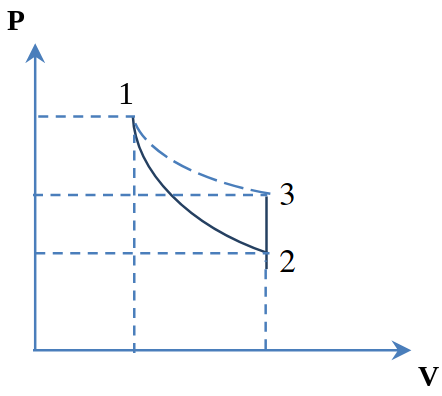
\includegraphics[scale=0.5]{1}
	\end{center}
	\caption{Диаграмма P--V}

\end{figure}
Метод Клемана-Дезорма основывается на изучении параметров некоторой массы газа, переходящей из одного состояния в другое двумя последовательными процессами: адиабатический и изохорический. Они изображены кривыми 1--2 и 2--3 соответственно на Рис. 1.

Если в баллон, соединённый с открытым водяным манометром, накачать воздух и подождать до установления теплового равновесия с окружающей средой, то в начальном состоянии газ имеет параметры $P_1, V_1, T_1$. При этом температура в баллоне равна температуре окружающей среды $T_1 = T_0$, а давление чуть болье атмосферного: $P_1 = P_0 + P'$. Если теперь на короткое время соединить баллон с
атмосферой, то произойдёт адиабатное расширение воздуха. При этом воздух в баллоне перейдёт в состояние 2, его давление
понизится до атмосферного $P_2 = P_0$. Масса воздуха, оставшегося в
баллоне, которая в состоянии 1 занимала часть объёма баллона,
расширяясь, займёт весь объём $V_2$ При этом температура воздуха,
оставшегося в баллоне, понизится до $T_2$.

Так как процесс 1--2 - адиабатический, к нему можно применить уравнение Пуассона \eqref{puasson}:
$$P_1V_1^\gamma = P_2V_2^\gamma$$
или
$$\frac{T_1^\gamma}{P_1^{\gamma-1}} = \frac{T_2^\gamma}{P_2^{\gamma-1}}$$
Отсюда
$$\bigg(\frac{P_0 + P'}{P_0}\bigg)^{\gamma-1} = \bigg(\frac{T_0}{T_2}\bigg)^{\gamma}$$

Затем воздух будет нагреваться (процесс 2--3) до температуры окружающей среды ($T_3 = T_0$) при постоянном объеме ($V_3 = V_2$). При этом давление в баллоне поднимется до $P_3 = P_0 + P''$.

$$\bigg(\frac{P_0 + P'}{P_0}\bigg)^{\gamma-1} = \bigg(\frac{P_0 + P''}{P_0}\bigg)^{\gamma} \rightarrow$$
$$\rightarrow (\gamma - 1)\ln\bigg(1+\frac{P'}{P_0}\bigg) = \gamma\ln\bigg(1+\frac{P''}{P_0}\bigg)$$

Так как избыточные давления $P'$ и $P''$ очень малы по сравнению с атмосферным давлением, можно разложить логарифмы в ряд Тейлора (ограничившись членами первого порядка малости). Получаем:
$$(\gamma-1)P' = \gamma P'' \rightarrow$$
$$\rightarrow \gamma = \frac{P'}{P' - P''}$$
Избыточные давления измеряются U-образным манометром по разности уровней жидкости с плотностью $\rho$:
$$P' = \rho gh_1; P'' = \rho g h_2$$.
Таким образом, получаем рабочую формулу:
\begin{equation}\label{rab_form}
\gamma = \frac{h_1}{h_1-h_2}
\end{equation}

\newpage
\section{Ход эксперимента}
\hspace{\parindent}В данной работе с помощью экспериментальной установки мы определили показатель адиабаты воздуха.

Экспериментальная установка представляет собой водяной манометр с тумблерами, необходимыми для регулировки контакта воды с атмосферой, а также накачивания воздуха.

Для начала мы проконтролировали, чтобы уровни воды в обоих коленах водяного манометра были равны. После чего, ограничив контакт жидкости с атмосферой, произвели накачку воздуха. Через небольшой промежуток времени подача воздуха прекращалась. На данном этапе нам было необходимо дождаться момента, когда уровни воды в обоих коленах придут в состояние покоя. После этого мы определили значение $h_1$, равное разности значений в соответствующих коленах.

После определения первой необходимой величины, мы \textbf{кратковременно} обеспечили контакт системы с атмосферой и провели аналогичные измерения для новых значений высот $h_2$.

Полученные результаты представлены ниже:
\begin{center}
	\begin{tabular}{|c|c|c|c|}
		\hline
		№&$(h_1 \pm \Delta h_1)$, 1 мм в.с.&$(h_2 \pm \Delta h_2)$, 1 мм в.с.&$(\gamma \pm \Delta\gamma)$
		\\ 
		\hline
		1	&178 ± 0,5	&45 ± 0,5		&1,338 ± 0,005
		\\
		\hline
		2	&149 ± 0,5	&52 ± 0,5		&1,536 ± 0,008
		\\
		\hline
		3	&142 ± 0,5	&35 ± 0,5		&1,327 ± 0,006
		\\
		\hline
		4	&202 ± 0,5	&53 ± 0,5		&1,355 ± 0,005
		\\
		\hline
		5	&167 ± 0,5	&47 ± 0,5		&1,391 ± 0,006
		\\
		\hline
		6	&174 ± 0,5	&43 ± 0,5		&1,328 ± 0,005
		\\
		\hline
		7	&183 ± 0,5	&51 ± 0,5		&1,386 ± 0,005
		\\
		\hline
		8	&203 ± 0,5	&60 ± 0,5		&1,419 ± 0,005
		\\
		\hline
		9	&211 ± 0,5	&74 ± 0,5		&1,540 ± 0,006
		\\
		\hline
		10	&159 ± 0,5	&44 ± 0,5		&1,382 ± 0,006
		\\
		\hline
	\end{tabular}
\end{center}
где 1 мм в.с. = 10Па.

Далее, используя рабочую формулу \eqref{rab_form}, мы определили значения показателя адиабаты для каждой серии измерений.

Среднее значение показателя адиабаты воздуха, исходя из данных, будет равно:
$$\gamma = 1,400$$

Данное значение с точностью до тысячных сходится с табличным значением показателя адиабаты сухого воздуха при $t = 20^\circ С$.

\newpage
\subsection{Погрешности измерений}
В данной работе будет фигурировать систематическая погрешность в определении значений $h_1, h_2$. А также косвенная погрешность в определении показателя адиабаты $\gamma$. Необходимые формулы представлены ниже:

$$\Delta h = \frac{ц.д.}{2}*\alpha,$$ 
где ц.д. -- цена деления шкалы, $\alpha$ -- доверительный интервал.
\vspace{0.5cm}
$$\Delta\gamma = \sqrt{\bigg(\frac{-h_2}{(h_1-h_2)^2}\Delta h_1\bigg)^2 + \bigg(\frac{h_1}{(h_1-h_2)^2}\Delta h_2\bigg)^2},$$
где $\Delta h_1$ -- систематическая погрешность $h_1$, $\Delta h_2$ -- систематическая погрешность $h_2$.

\newpage
\section{Вывод}
\hspace{\parindent}Целью данной работы являлось определение показателя адиабаты методом Клемана-Дезорма, суть которого заключается в переходе к более удобным для вычисления переменным, а именно -- высотам. 

Определение показателя адиабаты не вызвало у нас каких-либо трудностей. Факт совпадения экспериментального значения с табличным означает, что эксперимент был проведён с высокой точностью.




\end{document}